\newpage
\section*{Problem 4:}
\begin{enumerate}
\item The function \texttt{nonsymmetric\_lanczos} implements the nonsymmetric Lanczos process where it takes a function that implements $Av$ and another function that implements $A^{T}v$ along with the initial $r$ and $c$ vectors. It outputs the $T_{k}$ tridiagonal matrix is sparse format. We used this function to compute $T_{k} $ for $K=5, 10, \text{\ and\ } 20$ and computed the eigenvalues of $T_{k}$. To compare between the eigenvalue of $T_{20}$ and $A$'s eigenvalues, we computed $\parallel A\_eig - T_{20}\_eig\parallel =\expnumber{6.448717}{-13}$


\begin{figure}[tbh]
 \centering    
\begin{tabular}{ |p{1cm}|| p{10cm}|}
\hline
 K & Eigenvalues \\ \hhline{|=|=|}   
\hline
5 & $\expnumber{-2.501781014189590}{+00 }  \expnumber{+ 5.900692650763462}{+00i}$\\
  & $\expnumber{-3.090333049113557}{+00 }  \expnumber{+ 4.825912738594896}{-01i}$\\
  & $\expnumber{ 5.172926282011777}{-01 }  \expnumber{- 7.888954236341315}{-01i}$\\
  & $\expnumber{ 1.256199307483214}{+00 }  \expnumber{- 3.493703520606647}{+00i}$\\
  & $\expnumber{ 1.274556869629201}{+01 }  \expnumber{- 1.125556172280826}{+01i}$\\
\hline  
10& $\expnumber{ 1.338852744862344}{-01}  \expnumber{- 3.681053207507567}{+00i}$\\
  & $\expnumber{ 2.508862893210253}{+00}  \expnumber{- 2.197729989474411}{+00i}$\\
  & $\expnumber{ 2.670866099884081}{+00}  \expnumber{- 1.314179550767412}{+00i}$\\
  & $\expnumber{-4.439295624831807}{-01}  \expnumber{- 2.347985483160573}{+00i}$\\
  & $\expnumber{-2.826197293664038}{+00}  \expnumber{- 2.998937801231081}{-01i}$\\
  & $\expnumber{-1.899586046943437}{+00}  \expnumber{+ 7.856568851355709}{-02i}$\\
  & $\expnumber{-2.187569680623757}{+00}  \expnumber{+ 2.082401070017189}{+00i}$\\
  & $\expnumber{-1.238832783943400}{+00}  \expnumber{+ 3.769011471476989}{+00i}$\\
  & $\expnumber{ 1.936757547900978}{+00}  \expnumber{+ 2.974410140200699}{+00i}$\\
  & $\expnumber{ 3.216278496510915}{+00}  \expnumber{+ 5.676288164244975}{+00i}$\\
\hline  
20& $\expnumber{-1.246365732148833}{+00}  \expnumber{+ 3.879484437687169}{+00i}$\\
  & $\expnumber{ 2.594180629560308}{+00}  \expnumber{- 2.284902242884396}{+00i}$\\
  & $\expnumber{-1.983514535906585}{+00}  \expnumber{+ 2.443522984313314}{+00i}$\\
  & $\expnumber{ 3.000394334727138}{+00}  \expnumber{- 9.028020730499668}{-01i}$\\
  & $\expnumber{-2.816575470153615}{+00}  \expnumber{- 4.470235401498108}{-01i}$\\
  & $\expnumber{ 2.304844231638672}{+00}  \expnumber{+ 1.654017825159949}{+00i}$\\
  & $\expnumber{-2.335649345045510}{+00}  \expnumber{+ 1.118762976889514}{+00i}$\\
  & $\expnumber{ 1.251730623491955}{-01}  \expnumber{- 3.705917327586384}{+00i}$\\
  & $\expnumber{-8.152087361523326}{-01}  \expnumber{- 2.850024263184126}{+00i}$\\
  & $\expnumber{ 4.970325872396055}{-01}  \expnumber{+ 2.729519259822502}{+00i}$\\
  & $\expnumber{-5.433637042723353}{-02}  \expnumber{- 2.946384869537706}{+00i}$\\
  & $\expnumber{ 1.282928255975401}{+00}  \expnumber{+ 2.519903189853295}{+00i}$\\
  & $\expnumber{ 1.564476048921003}{+00}  \expnumber{+ 1.768834378822957}{+00i}$\\
  & $\expnumber{-1.643042886688555}{+00}  \expnumber{- 1.212344348158034}{+00i}$\\
  & $\expnumber{ 1.943119133724864}{+00}  \expnumber{+ 8.605877308030484}{-02i}$\\
  & $\expnumber{ 1.486930904640041}{-01}  \expnumber{- 1.861577918840281}{+00i}$\\
  & $\expnumber{-1.013702946373266}{+00}  \expnumber{- 2.443176161667233}{-01i}$\\
  & $\expnumber{-4.328984355639987}{-01}  \expnumber{+ 1.008036318652911}{+00i}$\\
  & $\expnumber{ 6.261926774054385}{-01}  \expnumber{- 5.762496449081425}{-01i}$\\
  & $\expnumber{ 4.487381899523429}{-01}  \expnumber{- 2.877609613824950}{-01i}$\\
\hline  
\end{tabular} 
\caption{$T_{k}$ Eigenvalues for different values of $K$}
   \label{tab:t_k_eig}
\end{figure} 

\item we used our  \texttt{nonsymmetric\_lanczos} and  \texttt{arnoldi\_process}  to find the converged eigenvalues for the matrix in file \texttt{HW4\_P4b.mat} for increasing values of $k$. We note that in out implementation we used the efficient matrix-vector multiplication routine developed in homework 3. It easy to use it to also implement transposed-matrix-vector multiplication needed for Lanczos process.


It was hard to track down numerically what are the converged eigenvalues for both method. However, plotting the eigenvalues of $A\textprime$ along with the eigenvalues of $T_{k}$ from the nonsymmetric Lanczos process and $H_{k}$ from Arnoldi process, we can easily see the converged eigenvalues. Figure~\ref{fig:ard} shows how eigenvalues converges for increasing values of $K$. We notice that for small values of $K$, nonsymmetric Lanczos has a better chance to get eigenvalues that are true eigenvalues. 

\item We used the same function and efficient matrix-vector multiplication to carry on this part. However, on personal laptop, nonsymmetric Lanczos runs of memory quickly even for small $K$ on the matrix provided on \texttt{HW4\_P4c.mat}. Thus, we used the same matrix as part (b) to show the correctness of our method for increasing $K$. Figure~\ref{fig:cc} shows the eigenvalues obtained for different $K$ values. We also computed the norm of difference between each consecutive step we took (after sorting the eigenvalues). Table~\ref{tab:err} shows these norm. While Figure~\ref{fig:cc} shows that the eigenvalues converges, the differences shown in~\ref{tab:err} does not correlate with this as the difference increases with increasing $K$. We think this is due to some outlier eigenvalues that can be seen along the x-axis. 

\begin{figure}[!tbh]
\centering        
   \subfloat[K= 20]{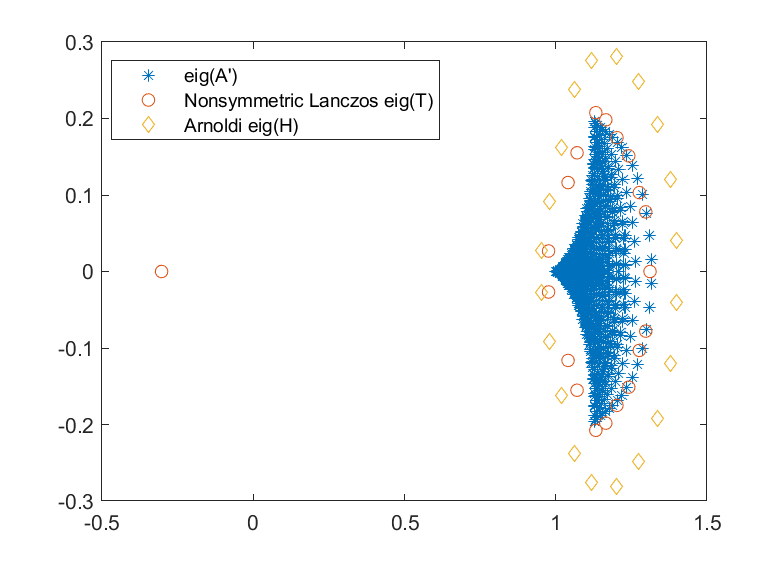
\includegraphics[width=0.52\textwidth]{../code/p4b_k_20.png}}
   \subfloat[K=60]{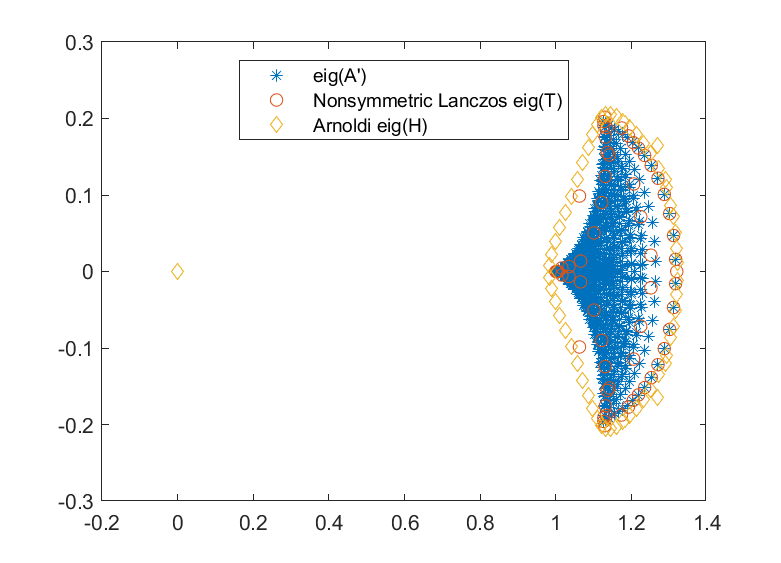
\includegraphics[width=0.52\textwidth]{../code/p4b_k_60.png}}
      
   \subfloat[K=100]{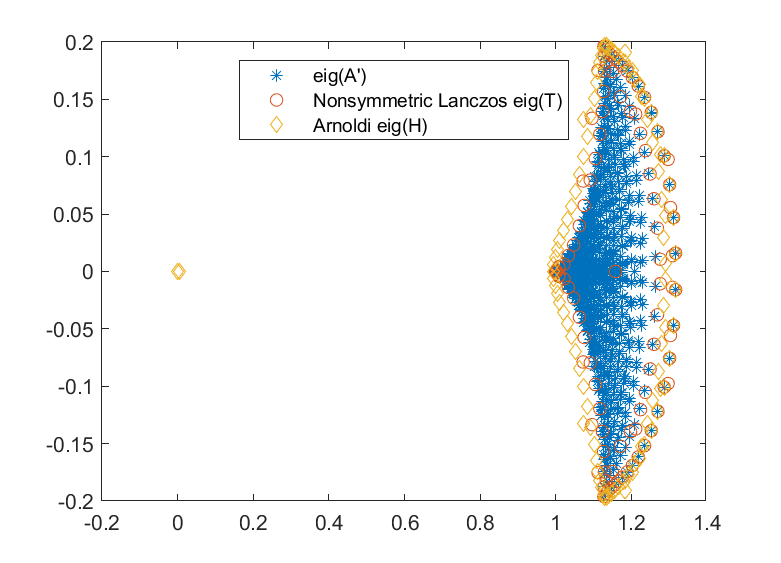
\includegraphics[width=0.52\textwidth]{../code/p4b_k_100.png}}    
   \subfloat[K=200]{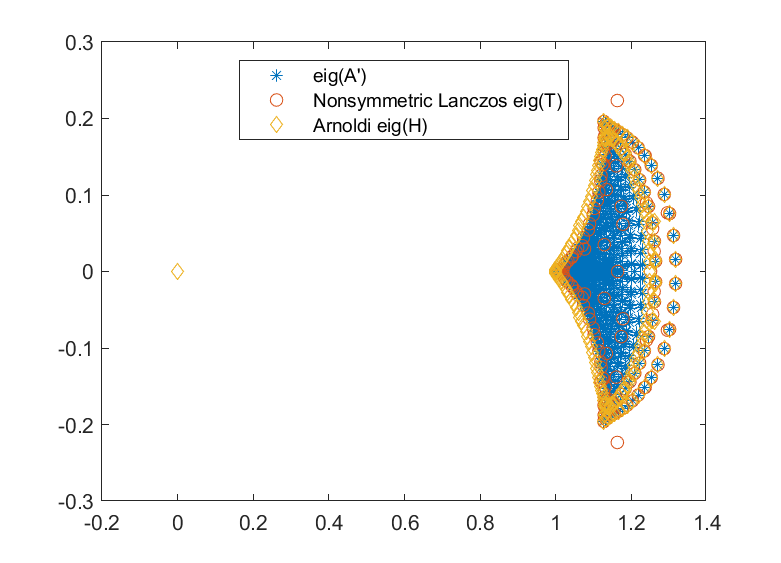
\includegraphics[width=0.52\textwidth]{../code/p4b_k_200.png}}
   
   \subfloat[K=300]{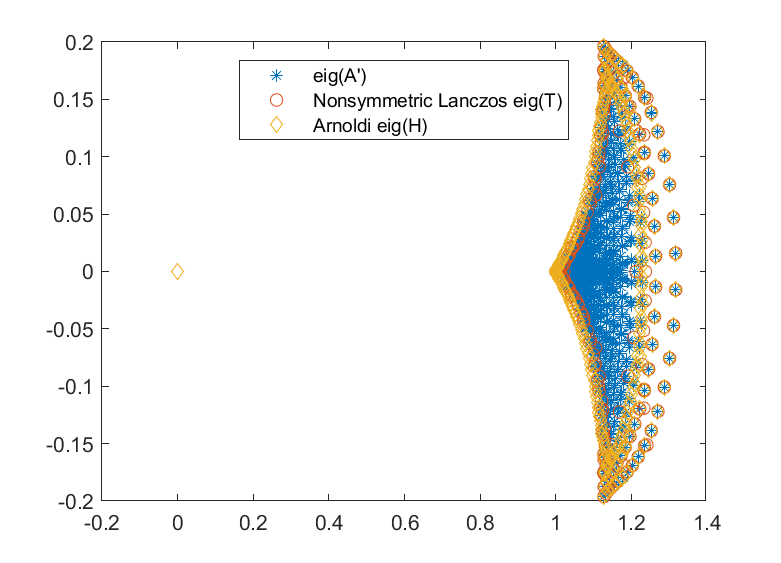
\includegraphics[width=0.52\textwidth]{../code/p4b_k_300.png}}
   \subfloat[K=500]{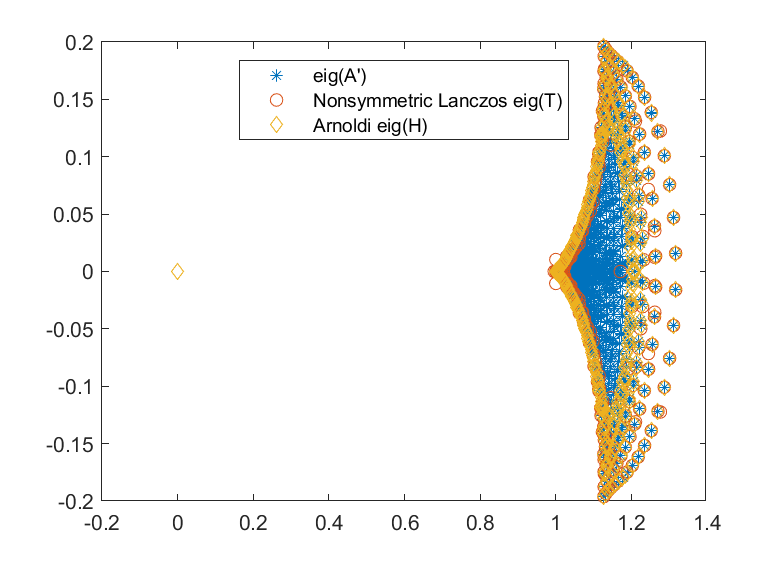
\includegraphics[width=0.52\textwidth]{../code/p4b_k_500.png}}
   
   \caption{Converged eigenvalues from nonsymmetric Lanczos and Arnoldi process.}
   \label{fig:ard}
\end{figure}




\begin{figure}[!tbh]
 \centering    
\begin{tabular}{ |p{1cm}|| p{10cm}|}
\hline
 K & Norm of the difference between eigenvalue of $T_{k}$  and $T_{k-1}$\\ \hhline{|=|=|}   
\hline
20 & \\
\hline  
60&	1.478839\\       
\hline  
100&	2.283969 \\       
\hline  
200&	1.590567 \\       
\hline  
300&	2.787656\\       
\hline  
500&	4.120523 \\       
\hline  
1000&	3.833748 \\       
\hline  
\end{tabular} 
\caption{The norm of the difference between the eigenvalues at $K$ and $K-1$ using for increasing values of $k$ of nonsymmetric Lanczos process}
   \label{tab:err}
\end{figure} 


\begin{figure}[!tbh]
\centering        
   \subfloat[K= 20]{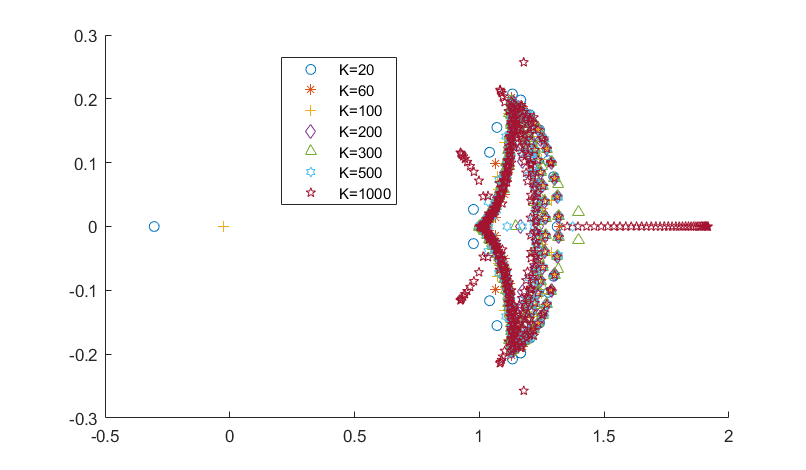
\includegraphics[width=0.9\textwidth]{../code/p4c.png}} 
   
   \caption{Eigenvalues obtain from nonsymmetric Lanczos for increasing value of $K$}
   \label{fig:cc}
\end{figure}


\end{enumerate}